
\begin{frame}
\begin{tabular}{lll}
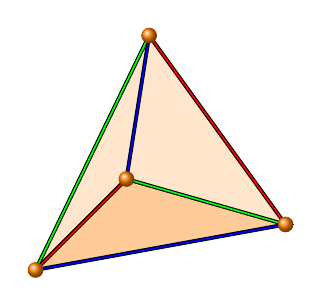
\begin{tikzpicture}[scale=3]
  \tikzset{VertexStyle/.style = {shape          = circle,
                                 ball color     = orange,
                                 text           = black,
                                 inner sep      = 2pt,
                                 outer sep      = 0pt,
                                 minimum size   = 4 pt}}
  \tikzset{EdgeStyleRed/.style   = {thin,
                                 double          = red}}
%                                 double distance = 1pt}}
  \tikzset{EdgeStyleBlue/.style   = {thin,
                                 double          = blue}}
%                                 double distance = 1pt}}
  \tikzset{EdgeStyleGreen/.style   = {thin,
                                 double          = green}}
%                                 double distance = 1pt}}

    \coordinate (A0) at (0,.8,0);
    \coordinate (AT) at (0.57735,0,0);
    \coordinate (AL) at (-0.288675,0,-.5);
    \coordinate (AR) at (-0.288675,0,0.5);
   \draw[fill=orange!40] (A0.center) -- (AT.center) -- (AR.center) -- cycle;
   \draw[fill=orange!20] (A0.center) -- (AT.center) -- (AL.center) -- cycle;
   \draw[fill=orange!20] (A0.center) -- (AL.center) -- (AR.center) -- cycle;
%   \draw[fill=orange!40] (AT.center) -- (AL.center) -- (AR.center) -- cycle;
    \draw[EdgeStyleRed] (A0.center) -- (AT.center);
    \draw[EdgeStyleBlue] (A0.center) -- (AL.center);
    \draw[EdgeStyleGreen] (A0.center) -- (AR.center);
    \draw[EdgeStyleRed] (AL.center) -- (AR.center);
    \draw[EdgeStyleGreen] (AL.center) -- (AT.center);
    \draw[EdgeStyleBlue] (AT.center) -- (AR.center);
   \draw (A0)  node[VertexStyle]  {};
   \draw (AT)  node[VertexStyle]  {};
   \draw (AL)  node[VertexStyle]  {};
   \draw (AR)  node[VertexStyle]  {};
\end{tikzpicture}
& &
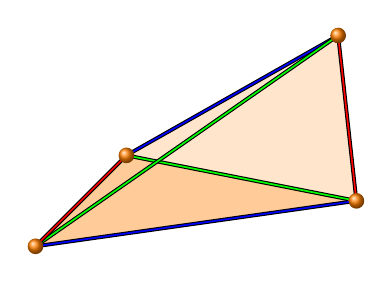
\begin{tikzpicture}[scale=3]
  \tikzset{VertexStyle/.style = {shape          = circle,
                                 ball color     = orange,
                                 text           = black,
                                 inner sep      = 2pt,
                                 outer sep      = 0pt,
                                 minimum size   = 4 pt}}
  \tikzset{EdgeStyleRed/.style   = {thin,
                                 double          = red}}
%                                 double distance = 1pt}}
  \tikzset{EdgeStyleBlue/.style   = {thin,
                                 double          = blue}}
%                                 double distance = 1pt}}
  \tikzset{EdgeStyleGreen/.style   = {thin,
                                 double          = green}}
%                                 double distance = 1pt}}

    \coordinate (A0) at (.8,0.7,0); % oben
    \coordinate (AT) at (0.87735,0,0); % rechts
    \coordinate (AL) at (-0.288675,0,-.5); %hinten
    \coordinate (AR) at (-0.288675,0,0.5); %links
%   \draw[fill=orange!40] (A0.center) -- (AT.center) -- (AR.center) -- cycle;
   \draw[fill=orange!20] (A0.center) -- (AT.center) -- (AL.center) -- cycle;
   \draw[fill=orange!20] (A0.center) -- (AL.center) -- (AR.center) -- cycle;
   \draw[fill=orange!40] (AT.center) -- (AL.center) -- (AR.center) -- cycle;
    \draw[EdgeStyleRed] (A0.center) -- (AT.center);
    \draw[EdgeStyleBlue] (A0.center) -- (AL.center);
    \draw[EdgeStyleGreen] (AL.center) -- (AT.center);
    \draw[EdgeStyleGreen] (A0.center) -- (AR.center);
    \draw[EdgeStyleRed] (AL.center) -- (AR.center);
    \draw[EdgeStyleBlue] (AT.center) -- (AR.center);
   \draw (A0)  node[VertexStyle]  {};
   \draw (AT)  node[VertexStyle]  {};
   \draw (AL)  node[VertexStyle]  {};
   \draw (AR)  node[VertexStyle]  {};
\end{tikzpicture}\\
A regular tetrahedron & &
A non-regular tetrahedron \\
with a wild colouring. & & with a wild colouring. 
\end{tabular}
\end{frame}

